\documentclass{article}

%\usepackage{hyperref}
\usepackage{url}
\usepackage{graphicx}
\usepackage[utf8]{inputenc}
%\usepackage{listings}
\usepackage[listings,skins,breakable,raster,most]{tcolorbox}
\usepackage{lstautogobble}
\usepackage{tabularx}
\usepackage{geometry}
\usepackage{hyperref}
\usepackage{cleveref}
\usepackage{silence}
\WarningFilter[]{latex}{File}
\WarningFilter[]{latex}{Unknown}



\geometry{margin=1.5in}

\lstset{ %
  autogobble=true,
  backgroundcolor=\color{black!5},   % choose the background color; you must add \usepackage{color} or \usepackage{xcolor}
  basicstyle=\normalfont\ttfamily,       % the size of the fonts that are used for the code
  breakatwhitespace=false,         % sets if automatic breaks should only happen at whitespace
  breaklines=true,                 % sets automatic line breaking
  captionpos=b,                    % sets the caption-position to bottom
  %commentstyle=\color{green},    % comment style
  deletekeywords={...},            % if you want to delete keywords from the given language
  escapeinside={(*@}{@*)},          % if you want to add LaTeX within your code
  extendedchars=true,              % lets you use non-ASCII characters; for 8-bits encodings only, does not work with UTF-8
  frame=none,	                   % (none, single) adds a frame around the code
  keepspaces=true,                 % keeps spaces in text, useful for keeping indentation of code (possibly needs columns=flexible)
  keywordstyle=\color{blue},       % keyword style
  language=C,                 % the language of the code
  otherkeywords={*,...},           % if you want to add more keywords to the set
  %numbers=left,                    % where to put the line-numbers; possible values are (none, left, right)
  numbersep=5pt,                   % how far the line-numbers are from the code
  numberstyle=\tiny\color{gray}, % the style that is used for the line-numbers
  rulecolor=\color{black},         % if not set, the frame-color may be changed on line-breaks within not-black text (e.g. comments (green here))
  showspaces=false,                % show spaces everywhere adding particular underscores; it overrides 'showstringspaces'
  showstringspaces=false,          % underline spaces within strings only
  showtabs=false,                  % show tabs within strings adding particular underscores
  stepnumber=1,                    % the step between two line-numbers. If it's 1, each line will be numbered
  stringstyle=\color{blue},     % string literal style
  tabsize=2,	                   % sets default tabsize to 2 spaces
  %title=\lstname                   % show the filename of files included with \lstinputlisting; also try caption instead of title
}

\title{ESDM Documentation}
\date{}
\author{}

\begin{document}

\maketitle

\tableofcontents

% INTRO
\section{Earth System Data Middleware}%
\label{earth-system-data-middleware}

The middleware for earth system data is a prototype to improve I/O
performance for earth system simulation as used in climate and weather
applications. ESDM exploits structural information exposed by workflows,
applications as well as data description formats such as HDF5 and NetCDF
to more efficiently organize metadata and data across a variety of
storage backends.

%\href{https://travis-ci.org/ESiWACE/esdm}{\includegraphics{https://travis-ci.org/ESiWACE/esdm.svg?branch=master}}

\subsection{Requirements}%
\label{requirements}

A compiler for C99 such as GCC5.0

\subsection{Installation}%
\label{installation}

Ensure you cloned the repository with the required submodules:

\begin{itemize}
  \item git clone -\/-recurse-submodules Or to initialize the submodules after the cloning:
  \item git submodule update -\/-init -\/-recursive
\end{itemize}

The installation instructions for the full stack with ESDM and NetCDF
can be found in the Dockerfiles that we use for testing.

\subsubsection{Ubuntu 20.04}%
\label{ubuntu-2004}

\$ grep RUN dev/docker/ubuntu-whole-stack/Dockerfile

\paragraph{Installation for CentOS7}%
\label{installation-for-centos7}

\$ grep RUN dev/docker/centos7-whole-stack/Dockerfile

\paragraph{Installation for FedoraSystem}%
\label{installation-for-fedora-system}

\begin{itemize}
  \item dnf install glib2 glib2-devel mpi jansson jansson-devel
  \item dnf install mpich-3.0 mpich-3.0-devel OR dnf install openmpi
    opemmpi-devel
  \item dnf install gcc-c++ gcc libtool cmake
\end{itemize}

\paragraph{Installation with Spack}%
\label{installation-with-spack}

Installation of spack itself:

\begin{itemize}
  \item git clone \url{https://github.com/spack/spack}
  \item export PATH=\$PATH:\$PWD/spack/bin/ Check that a suitable compiler is
    found
  \item spack compilers
\end{itemize}

First get the recent GCC:

\begin{itemize}
  \item spack install \href{mailto:gcc@9.3.0}{\nolinkurl{gcc@9.3.0}} Then
    install the packages with GCC:
  \item spack install jansson\%\href{mailto:gcc@9.3.0}{\nolinkurl{gcc@9.3.0}}
    glib\%\href{mailto:gcc@9.3.0}{\nolinkurl{gcc@9.3.0}}
    openmpi\%\href{mailto:gcc@9.3.0}{\nolinkurl{gcc@9.3.0}}
    gettext\%\href{mailto:gcc@9.3.0}{\nolinkurl{gcc@9.3.0}} Before running
    configure load the modules:
  \item spack load jansson\%\href{mailto:gcc@9.3.0}{\nolinkurl{gcc@9.3.0}}
    glib\%\href{mailto:gcc@9.3.0}{\nolinkurl{gcc@9.3.0}}
    openmpi\%\href{mailto:gcc@9.3.0}{\nolinkurl{gcc@9.3.0}} gcc
    gettext\%\href{mailto:gcc@9.3.0}{\nolinkurl{gcc@9.3.0}} -r
\end{itemize}

\subsection{Development}%
\label{development}

\subsubsection{Project directory structure}%
\label{project-directory-structure}

\begin{itemize}
  \item \texttt{dev} contains helpers for development purposes. For example,
    this project requires a development variant of HDF5 that provides the
    Virtual Object Layer (VOL). This and other dependencies can be
    installed into a development environment using the following script:

    \begin{lstlisting}
    ./dev/setup-development-environment.sh
    \end{lstlisting}
  \item \texttt{src} contains the source code... To build the project call:

    \begin{lstlisting}
    source dev/activate-development-environment.bash
    ./configure --debug
    cd build
    make -j
    \end{lstlisting}

    To run the test suite call:

    \begin{lstlisting}
    cd build
    make test
    \end{lstlisting}

    You may also choose to configure with a different hdf5 installation
    (see ./configure -\/-help) e.g.:

    \begin{lstlisting}
    ./configure --with-hdf5=$PWD/install
    \end{lstlisting}
  \item \texttt{doc} contains documentation which uses doxygen to build a HTML
    or a PDF version:

    For the HTML Reference use the following commands (assuming
    ./configure completed successfully):

    \begin{lstlisting}
    cd build
    doxygen
    build/doc/html/index.html
    \end{lstlisting}

    For a PDF Reference (requries LaTeX) run:

    \begin{lstlisting}
    cd build
    doxygen
    cd /doc/latex
    make
    \end{lstlisting}
  \item \texttt{tools} contains separate programs, e.g., for benchmarking
    HDF5. They should only be loosely coupled with the source code and
    allow to be used with the regular HDF5.
\end{itemize}

\section{Documentation}

\begin{figure}[!ht]
  \begin{center}
    \includegraphics[width=\textwidth]{../assets/build-docs-overview/graph.png}
  \end{center}
  \caption{Conversion paths.}
  \label{fig:build-docs-overview}
\end{figure}

The documentation is organized as a set of latex and resource files.
This structure simplifies integration in other documents if only particular documentation parts are required.
The source files are located in \lstinline|./doc/latex|.
This is a central location where files can be modified if changes are required.
All other locations listed in these sections are auto-generated.
Therefore, after recompilation all changes will be overwritten.

Documentation centralization reduces documentation efforts.
Changes in the latex files will affect all other auto-generated documents.
As shown in \Cref{fig:build-docs-overview}, the latex source files are exported to PDF, Github-Markdown, Latex and HTML formats.
PDF and Github-Markdown don't include ESDM-API reference.
You find it in the Latex and HTML generated by Doxygen.

The \Cref{code:doc:latex,code:dox:doxy-markdown,code:doc:doxygen,code:doc:doxygen:pdf,code:doc:gfm} in this section assume that current working directory is the ESDM repository.
The subsections discuss the supported export possibilities in detail.

\subsection{PDF}
Latex documentation can be compiled to a PDF file by commands shown in \Cref{code:doc:latex}.
The result will be stored in \lstinline|./doc/latex/main.pdf|

\begin{lstlisting}[caption={Make PDF document},label={code:doc:latex}]
cd ./doc
make
\end{lstlisting}

\subsection{Github-Markdown}
The Github documentation \lstinline|./README.md| is generated by \lstinline|pandoc| from the \lstinline|./doc/latex/main.tex| file.
%\lstinline|pandoc| uses a lua-filter (\lstinline|./doc/latex/image-path-filter.lua|) to change the paths to resource files.
\lstinline|./README.md| should never be modified manually since the next documentation compilation will overwrite changes.
The compilation commands are shown in \Cref{code:doc:gfm}.

\begin{lstlisting}[caption={Make ./README.md},label={code:doc:gfm}]
cd ./doc
make
\end{lstlisting}

\subsection{HTML and Latex with API reference}
Doxygen depends on a set of auto-generated markdown files, which should never be modified manually because the next compilation will overwrite all changes.
Please always work with files in \lstinline|./doc/latex| folder and compile them running the make script as shown in \Cref{code:dox:doxy-markdown}.

\begin{lstlisting}[caption={Markdown files generation},label={code:dox:doxy-markdown}]
cd ./doc
make
\end{lstlisting}

The resulting \lstinline|*.md| files are generated in \lstinline|./doc/markdown| directory.
Now all required source files for Doxygen should be available, and the final documentation can be compiled by \lstinline|doxygen| as shown in \Cref{code:doc:doxygen}.

\begin{lstlisting}[caption={Make HTML and Latex documents},label={code:doc:doxygen}]
./configure
cd build
doxygen
\end{lstlisting}

The resulting HTML start page is located in \lstinline|./build/doc/html/index.html|, and the main Latex document is located in \lstinline|./build/doc/latex/refman.tex|.

\begin{lstlisting}[caption={Comple PDF with API reference},label={code:doc:doxygen:pdf}]
cd doc/latex
pdflatex refman.tex
\end{lstlisting}

The resulting PDF file is \lstinline|./build/doc/latex/refman.pdf|



% MODEL
\section{Data model}%
\label{data-model}
%While datatypes introduced by computer architectures and software libraries are important for the data model, they are discussed separately in \eb{Reference}.

The data model of a system organizes elements of data, standardizes how they represent data entities and how users can interact with the data.
The \textbf{model} can be split into three layers:

\begin{itemize}
  \item The \textbf{conceptual data} model describes the entities and the semantics of the domain that are represented by the data model and the typical operations to manipulate the data. 
    In our case, the scientific domain is numerical weather prediction and climate.
  \item The \textbf{logical data model} describes the abstraction level provided by the system, how domain entities are mapped to objects provided by the system\footnote{A entity of the domain model such as a car could be mapped to one or several objects.}, and the supported operations to access and manipulate these objects are defined.
    Importantly, the \textbf{logical data model} defines the semantics when using the operations to access and manipulate the system objects.
    For example, a system object of a relational model is a table -- representing attributes of a set of objects -- and a row of a table representing attributes of a single object.
  \item The physical data model describes how the logical entities are finally mapped to objects/files/regions on available hardware. 
    The physical data model is partly covered by the backends of ESDM, therefore, the descriptions will stop at that abstraction level.
\end{itemize}

\subsection{Conceptual data model}

Our conceptual data model is aligned with the needs of domain scientists from climate and weather. 
It reuses and extends from concepts introduced in a data model proposed for the Climate and Forecasting conventions for NetCDF data~\cite{gmd-10-4619-2017}.

\paragraph{Variable:}%
\label{variable}

A variable, \(V\), defines a set of data representing a discrete (generally scalar) quantity discretised within a ``sampling'' domain, \(d\). It is accompanied by metadata.

\paragraph{Metadata:}%
\label{metadata}

Which will include at the minimum, a name, but may also include units, and information about additional dimensionality, directly (e.g.~via a key, value pair such as that necessary to expose \(z=1.5m\) for air temperature at 1.5m) or indirectly (e.g.~via pointers to other generic coordinate variables which describe the sampled domain). 
There may also be a dictionary of additional metadata which may or may not conform to an external semantic convention or standard. 
Such metadata could include information about the tool used to observe or simulate the specific variable. 
Additional metadata is also required for all the other entities described below.

\paragraph{Dimension:}%
\label{dimension}

The sampling domain \(d\) is defined by dimensions which define an a coordinate axis. 
Dimensions will also include metadata, which must again, include at a minimum a name (e.g.~height, time), but may also include information about directionality, units (e.g.~degrees, months, days-since-a-particular-time-using-a-particular-calendar), or details of how to construct an algorithm to find the actual sampling coordinates, perhaps using a well known algorithm such as an ISO 8601 time.

\paragraph{Coordinate:}%
\label{coordinate}

Coordinates are the set of values at which data is sampled along any given dimension. 
They may be explicitly defined by indexing into a coordinate variable, or implicitly defined by an algorithm. 
When we talk about the coordinates, it is usually clear if we mean the N-dimensional coordinate to address data in a given variable or if we just mean the (1D) coordinate along one dimension.

\paragraph{Cell:}%
\label{cell}

The data values are known at points, which may or may not represent a cell. 
Such cells are n-dimensional shapes where the dimensionality may or may not fully encompass the dimensionality of the domain.
n-dimensional shapes can be implicitly defined in which case the Cartesian product of all dimensional coordinates forms the data "cube" of the cell, but they can also be explicitly defined, either by providing bounds on the coordinate variables (via metadata) or by introducing a new variable which explicitly defines the functional boundaries of the cell (as might happen in a finite element unstructured
grid).

\paragraph{Dataset:}%
\label{dataset}

Variables can be aggregated into datasets. 
A dataset contains multiple variables that logically belong together, and should be associated with metadata describing the reason for the aggregation. 
Variables must have unique names within a dataset.

Our conceptual model assumes that all variables are scalars, but clearly to make use of these scalars requires more complex interpretation. 
In particular, we need to know the datype and operators.
%\eb{Fix this}

\paragraph{Datatype:}%
\label{datatype}

defines the types of values that are valid and the operations that can be conducted. 
While we are mostly dealing with scalars, they may not be amenable to interpretation as simple numbers. 
For example, a variable may be storing an integer which points into a taxonomy of categories of land-surface-types. 
More complex structures could include complex data types such as vectors, compressed ensemble values, or structures within this system, provided such interpretation is handled outside of the ESDM, and documented in metadata. 
This allows us to limit ourselves to simple data types plus arbitrary length blocks of bits.

\paragraph{Operators:}%
\label{operators}

define the manipulations possible on the conceptual entities.
The simplest operators will include creation, read, update and delete applied to an entity as a whole, or to a subset, however even these simple operators will come with constraints, for example, it should not be possible to delete a coordinate variable without deleting the parent variable as well.
There will need to be a separation of concerns between operators which can be handled within the ESDM subsystem, and those which require external logic.
Operators which might require external logic could include subsetting --- it will be seen that the ESDM will support simple subsetting using simple coordinates --- but complex subsets such as finding a region in real space from dimensions spanned using an algorithm or coordinate variable, may require knowledge of how such algorithms or variables are specified.
Such knowledge is embedded in conventions such as the CF NetCDF conventions, and this knowledge could only be provided to the ESDM via appropriate operator plugins.
 
\subsection{Logical data model}

The logical data model describes how data is represented inside ESDM, the operations to interact with the data and their semantics.
There are four first class entities in the ESDM logical data model: \textbf{variable}s, \textbf{fragment}s, \textbf{container}s, and \textbf{metadata}.
ESDM entities may be linked by ESDM \textbf{reference}s, and a key property which emerges from the use of references is that no ESDM entity instance may be deleted while references to it still exist.
The use of reference counting will ensure this property as well as avoid dangling pointers.
 
%gives an overview of the logical data model.
%\eb{Fix this}

Each of these entities is now described, along with a list of supported operations:

\paragraph{Variable:}%
\label{variable-1}

In the logical data model, the variable corresponds directly to a variable in the conceptual data model.
Each element of the variable sampled across the dimensions contains data with a prescribed \textbf{DataType}.
Variables are associated with both \textbf{Scientific Metadata} and \textbf{Technical Metadata}.
Variables are partitioned into \textbf{fragments} each of which can be stored on one or more ``storage backend''.
A variable definition includes internal information about the domain (bounding box in some coordinate system) and dimensionality (size and shape), while the detailed information about which coordinate variables are needed to span the dimensions and how they are defined is held in the technical metadata.
Similarly, where a variable is itself a coordinate variable, a link to the parent variable for which it is used is held in the technical metadata.
The ESDM will not allow an attempt to delete a variable to succeed while any such references exist (see references).
A key part of the variable definition is the list of fragments associated with it, and if possible, how they are organised to span the domain.
Users may choose to submit code pieces that are then run within the I/O-path (not part within ESiWACE implementation), such an operation covers the typical filter, map and reduce operations of the data flow programming paradigm.
 
Fragments are created by the backend while appending/modifying data to a variable.

Operations:

\begin{itemize}
  \item Variables can be created and deleted.
  \item Fragments of data can be attached and deleted.
  \item Fragments can be repartitioned and reshuffled.
  \item Integrity can be checked.
  \item Data can be read, appended or modified those operations will be translated to the responsible fragments.
  \item Metadata can be atomically attached to a variable or modified.
  \item A variable can be sealed to make it immutable for all subsequent modifications.
  \item Process data of the variable somewhere in the I/O-path.
\end{itemize}

\paragraph{Fragment:}%
\label{fragment}

A fragment is a piece (subdomain) of a variable.
The ESDM expects to handle fragments as atomic entities, that is, only one process can write a fragment through the ESDM, and the ESDM will write fragments as atomic entities to storage backends.
The backends are free to further partition these fragments in an appropriate way, for example, by sharding using chunks as described in the mapping section.
However, the ESDM is free to replicate fragments or subsets of fragments and to choose which backend is appropriate for any given fragment.
This allows, for example, the ESDM to split a variable into fragments some of which are on stored on a parallel file system, while others are placed in object storage.
 
Operations:

\begin{itemize}
  \item Data of fragments can be read, appended or modified.
  \item Integrity of the fragment can be checked.
  \item Process data of the variable somewhere in the I/O-path.
\end{itemize}

\paragraph{Container:}%
\label{container}

A container is a virtual entity providing views on collections of variables, allowing multiple different datasets (as defined in the conceptual model) to be realised over the variables visible to the ESDM.
Each container provides a hierarchical namespace holding references to one or multiple variables together with metadata.
Variables cannot be deleted while they are referenced by a container.
The use of these dynamic containers provides support for much more flexible organisation of data than provided by a regular file system semantics --- and efficiently support high level applications such as the Data Reference Syntax~\cite{drs2012}.
 
A container provides the ESDM storage abstraction which is analogous to an external file.
Because many scientific metadata conventions are based on semantic structures which span variables within a file in ways that may be opaque to the ESDM without the use of a plugin, the use of a container can indicate to the ESDM that these variables are linked even though the ESDM does not understand why, and so they cannot be independently deleted.
When entire files in NetCDF format are ingested into the ESDM, the respective importing tool must create a container to ensure such linking properties are not lost.
 
Operations:

\begin{itemize}
  \item Creation and deletion of containers.
  \item Creation and deletion of names in the hierarchical name space; the creation of links to an existing variable.
  \item Attaching and modification of metadata.
  \item Integrity can be checked.
\end{itemize}

\paragraph{Metadata:}%
\label{metadata-1}

Can be associated with all the other first class entities (variables, fragments, and containers). Such metadata is split into internal ESDM technical metadata, and external user-supplied semantic metadata.

Technical metadata covers, e.g., permissions, information about data location and timestamps.
A backend will be able to add its own metadata to provide the information to lookup the data for the fragment from the storage backend managed by it.
Metadata by itself is treaded like a normal ESDM variable but linked to the variable of choice.
The implementation may embed (simple) metadata into fragments of original data (see Reference).
 
Operations:

\begin{itemize}
  \item Users can create, read, or delete arbitrary scientific metadata onto variables and containers. A future version of the ESDM may support user scientific metadata for fragments.
  \item Container level metadata is generally not directly associated with variables, but may be retrieved via following references from variables to containers.
  \item Queries allow to search for arbitrary metadata, e.g., for objects that have (\texttt{experiment=X}, \texttt{model=Y}, \texttt{time=yesterday}) returning the variables and containers in a list that match. This enables to locate scientific data in an arbitrary namespace.
\end{itemize}

\paragraph{Reference:}%
\label{reference}

A reference is a link between entities and can be used in many places, references can be embedded instead of real data of these logical objects.
For example, dimensions inside a variable can be references, also a container typically uses references to variables.
 
Operations:

\begin{itemize}
  \item A reference can be created from existing logical entities or removed.
\end{itemize}

%\begin{figure}
%  \centering
%  \includegraphics[width=0.5\textwidth]{../figures/data-model.png}
%  \caption{Logical Data Model (TODO)}%
%  \label{fig:data-model}
%\end{figure}

\paragraph{Namespace:}%
\label{namespace}

ESDM does not offer a simple hierarchical namespace for the files.
It provides the elementary functions to navigate data: teleportation and orientation in the following fashion: Queries about semantical data properties (e.g., \texttt{experiment=myExperiment}, \texttt{model=myModel}, \texttt{date=yesterday}) can be performed returning a list of matching files with their respective metadata.
Iterating the list (orientation) is similar to listing a directory in a file system.
 
Note that this reduces the burden to define a hierarchical namespace and for data sharing services based on scientific metadata.
An input/output container for an application can be assembled on-the-fly by using queries and name the resulting entities.
As a container provides a hierachical namespace, by harnessing this capability one can search for relevant variables and map them into the local file system tree, accessing these variables as if they would be, e.g., NetCDF files.
By offering a FUSE client, this feature also enables backwards compatibility for legacy POSIX applications.
 


% USER
\subsection{The ESDM Configuration File}

%\begin{figure}
%  \centering
%  \includegraphics[width=0.9\textwidth]{figures/data-model.png}
%  \caption{Dummy figure}
%  \label{fig:dummy}
%\end{figure}

\subsubsection{Search Paths}

TODO

\subsubsection{File Format}

The configuration file format is based on JSON, i.e. all configuration files must be valid JSON files.
However, ESDM places some restrictions on what keys are recognized and which types are expected.
The tables summarize parameters that can be used in the configuration file.
Parameter can be of four types: string, integer, float and object, which are collections of key-value pairs.

The ```"esdm":{}``` key-value pair in the root of the JSON configuration file can contain configuration for multiple data backends and one metadata backend.
The backends are organized in the ```backends``` key-value pair as a list.

\begin{lstlisting}
{
  "esdm":	{
    "backends": [backend_1, backend_2, \ldots, backend_n],
    "metadata": {}
  }
}
\end{lstlisting}


\begin{table}[!h]
  \centering
  \begin{tabularx}{\textwidth}{llllX}
  Parameter              & Type    & Default    &          & Description \\
  \hline
  type                   & string  & (not set)  & required & Backend name (see \Cref{tab:supported_backends}) \\
  id                     & string  & (not set)  & required & Unique identifier string \\
  target                 & string  & (not set)  & required & Connection specification (Bucket name for S3) \\
  performance-model      & object  & (not set)  & optional & Performance model definition. (see \Cref{tab:dyn_perf_model_conf_params,tab:gen_perf_model_conf_params}) \\
  max-threads-per-node   & integer & 0          & optional & Maximum number of threads on a node. \\
  write-stream-blocksize & integer & 0          & optional & TODO. \\
  max-global-threads     & integer & 0          & optional & Maximum total number of threads. \\
  accessibility          & string  & global     & optional & TODO. (see \Cref{tab:accessibility}) \\
  max-fragment-size      & integer & 10485760   & optional & Maximum fragment size in bytes. \\
  fragmentation-method   & string  & contiguous & optional & Fragmentation methods. (see \Cref{tab:frag_methods}) \\
  % S3 parameters
  host                   & string  & (not set)  & required & (S3 only) TODO \\
  secret-key             & string  & (not set)  & required & (S3 only) TODO \\
  access-key             & string  & (not set)  & required & (S3 only) TODO \\
  locationConstraint     & string  & (not set)  & required & (S3 only) TODO \\
  authRegion             & string  & (not set)  & required & (S3 only) TODO \\
  timeout                & integer & (not set)  & required & (S3 only) TODO \\
  s3-compatible          & integer & (not set)  & required & (S3 only) TODO \\
  use-ssl                & integer & 0          & required & (S3 only) TODO \\
  \end{tabularx}
  \caption{Backend configuration parameters}%
  \label{tab:backend_conf_params}
\end{table}




\paragraph{Parameter: id}
Unique identifier string.


\paragraph{Parameter: type and target}
Can take a value of one of the supported backends listed in @tbl:supportedtypes.

\begin{table}[!h]
  \centering
  \begin{tabular}{ll}
    Type   & Description                     \\ 
    \hline
    CLOVIS & Seagate Object Storage API      \\ 
    DUMMY  & (Used for development)          \\ 
    IME    & DDN Infinite Memory Engine      \\ 
    KDSA   & Kove Direct System Architecture \\ 
    POSIX  & POSIX interface                 \\ 
    S3     & Amazon Simple Storage Service   \\ 
    WOS    & DDN Object Storage              \\ 
  \end{tabular}
  \caption{Supported backends}%
  \label{tab:supported_backends}
\end{table}

\subparagraph{type = MOTR}

\begin{lstlisting} 
[local_addr] [ha_addr] [prof] [proc_fid]
\end{lstlisting}

  where
  \begin{itemize}
    \item "local\_addr" is the local address used to connect to Motr service, 
    \item "ha\_addr" is the hardware address in Motr service, 
    \item "prof" is the profile FID in the Motr service, and
    \item "proc\_fid" is the process FID in the Motr service.
  \end{itemize}
  
  \begin{lstlisting} 
  {
   "type": "MOTR",
   "id": "c1",
   "target": ":12345:33:103 192.168.168.146@tcp:12345:34:1 
     <0x7000000000000001:0> <0x7200000000000001:64>"
  }
  \end{lstlisting}
        
\subparagraph{type = DUMMY}

(Used for development)

\subparagraph{type = IME}
  TODO

  \begin{lstlisting}
  {
   "type": "IME",
   "id": "p1",
   "target": "./_ime"
  }
  \end{lstlisting}

\subparagraph{type = KDSA}

Prefix ``xpd:'' followed by volume specifications. Multiple volume names can be connected by ``+'' sign.

\begin{lstlisting}
xpd:mlx5\_0.1/260535867639876.9:e58c053d-ac6b-4973-9722-cf932843fe4e[+mlx...]
\end{lstlisting}

A module specification consists of several parts.
Caller provides a device handle, the target serial number, the target link number, the volume UUID,
The convention for specifying a KDSA volume uses the following format:

\begin{lstlisting}
[localdevice[.localport]/][serialnumber[.linknum]:]volumeid
\end{lstlisting}

where the square brackets indicate optional parts of the volume connection specification.
Thus, a volumeid is nominally sufficient to specify a desired volume, and one can then optionally additionally 
specify the serial number of the XPD with optional link number, and/or one can optionally specify the local 
device to use with optional local port number.
The convention for specifying multiple KDSA volumes to stripe together uses the following format:

\begin{lstlisting}
volume_specifier[+volume_specifier[+volume_specifier[+...]]][@parameter]
\end{lstlisting}

where the square brackets indicate optional parts of the aggregated connection specification. Thus, a single
volume connection specification is sufficient for a full connection specifier, and one can then optionally specify
additional volume specifiers to aggregate, using the plus sign as a separator. The user may also additionally
specify parameters for the aggregation, using the “at sign”, a single character as a parameter identifier, and the
parameter value.

\begin{lstlisting}
{
"type": "KDSA",
"id": "p1",
"target": "This is the XPD connection string",
"max-threads-per-node" : 0,
"max-fragment-size" : 1048,
"accessibility" : "global"
}
\end{lstlisting}

\subparagraph{POSIX}

Path to a directory, e.g., /home/user/data/

\begin{lstlisting}
{
 "type": "POSIX",
 "id": "p2",
 "target": "./_posix2"
}
\end{lstlisting}

\subparagraph{S3}
Bucket name prefix (at least 5 characters long)

\begin{table}[!h]
  \centering
  \begin{tabularx}{\textwidth}{llllX}
  Parameter              & Type    & Default    &          & Description \\
  \hline
  host                   & string  & (not set)  & required & (S3 only) TODO \\
  secret-key             & string  & (not set)  & required & (S3 only) TODO \\
  access-key             & string  & (not set)  & required & (S3 only) TODO \\
  locationConstraint     & string  & (not set)  & required & (S3 only) TODO \\
  authRegion             & string  & (not set)  & required & (S3 only) TODO \\
  timeout                & integer & (not set)  & required & (S3 only) TODO \\
  s3-compatible          & integer & (not set)  & required & (S3 only) TODO \\
  use-ssl                & integer & 0          & required & (S3 only) TODO \\
  \end{tabularx}
  \caption{S3 parameters}%
  \label{tab:s3_params}
\end{table}

TODO example

\subparagraph{WOS}
TODO

\begin{lstlisting}
{
"type": "WOS",
"id": "w1",
"target": "host=192.168.80.33;policy=test;",
"max-threads-per-node" : 1,
"max-fragment-size" : 1073741825,
"max-global-threads" : 1,
"accessibility" : "global"
}
\end{lstlisting}


\subparagraph{Parameter: performance-model}


\begin{table}[!ht]
  \centering
  \begin{tabularx}{\textwidth}{lllllX}
    Parameter  & Type  & Default & Domain &          & Description \\ 
    \hline
    latency    & float & 0.0     & >=0.0  & optional & seconds     \\ 
    throughput & float & 0.0     & >0.0   & optional & MiB/s       \\ 
  \end{tabularx}
  \caption{Dynamic performance model parameters}%
  \label{tab:dyn_perf_model_conf_params}
\end{table}


\begin{table}[!ht]
  \centering
  \begin{tabularx}{\textwidth}{lllllX}
    Parameter  & Type    & Default & Domain &          & Description         \\ 
    \hline
    latency    & float   & 0.0     & >=0.0  & optional & Latency in seconds  \\ 
    throughput & float   & 0.0     & >0.0   & optional & Throughput in MiB/s \\ 
    size       & integer & 0       & >0     & optional & TODO                \\ 
    period     & float   & 0.0     & >0.0   & optional & TODO                \\ 
    alpha      & float   & 0.0     & [0.0,  & 1.0)     & optional TODO       \\ 
  \end{tabularx}
  \caption{Generic performance model parameters}%
  \label{tab:gen_perf_model_conf_params}
\end{table}



\subparagraph{Parameter: max-threads-per-node}
TODO

\subparagraph{Parameter: write-stream-blocksize}
TODO

\subparagraph{Parameter: max-global-threads}
TODO

\subparagraph{Parameter: accessibility}

\begin{table}[!ht]
  \centering
  \begin{tabularx}{\textwidth}{lX}
    Method & Description \\ 
    \hline
    global & TODO        \\ 
    local  & TODO        \\ 
  \end{tabularx}
  \caption{Accessibility}%
  \label{tab:accessibility}
\end{table}

\subparagraph{Parameter: max-fragment-size}
The amount of data that may be written into a single fragment. 
The amount is given in bytes.

\subparagraph{Parameter: fragmentation-method}
A string identifying the algorithm to use to split a chunk of data into fragments. 
Legal values are:

\begin{table}[!ht]
  \centering
  \begin{tabularx}{\textwidth}{lX}
Method     & Description \\
\hline
contiguous  & This algorithm tries to form fragments that are 
            scattered across memory as little as possible. As such, 
            it is expected to yield the best possible write performance. 
            However, if a transposition is performed when reading 
            the data back, performance may be poor.
            Splitting a dataspace of size (50, 80, 100) into fragments 
            of 2000 entries results in fragments of size (1, 20, 100). \\
equalized   & This algorithm tries to form fragments that have a similar 
            size in all dimensions. As such, it is expected to perform 
            equally well with all kinds of read requests, but it tends 
            to write scattered data to disk which has to be sequentialized 
            first, imposing a performance penalty on the write side.
            Splitting a dataspace of size (50, 80, 100) into fragments of at
            most 2000 entries results in fragments of sizes between 
            (10, 11, 11) and (10, 12, 12). \\
  \end{tabularx}
  \caption{Fragmentation methods}%
  \label{tab:frag_methods}
\end{table}


\subsubsection{Metadata}
\begin{table}[!ht]
  \centering
  \begin{tabularx}{\textwidth}{lllX}
    Parameter & Type   & Default   & Description     \\ 
    \hline
    type      & string & (not set) & required TODO   \\ 
    id        & string & (not set) & (not used) TODO \\ 
  \end{tabularx}
  \caption{Metadata parameters}%
  \label{tab:metadata_params}
\end{table}


\section{Installation Instructions for Mistral}%
\label{installation-instructions-for-mistral}

Mistral (HLRE-3) is the supercomputer installed at DKRZ in 2015/2016.
This guide documents installation procedures to build prerequisites as
well as the prototype code base for development purposes.

\subsection{Satisfying Requirements}%
\label{satisfying-requirements}

Mistral offers users a number of software packages via the module
command (man module). While large parts of ESDM will build with the
standard tools available on the platform, it is still recommended to use
Spack \url{https://spack.readthedocs.io/en/latest/index.html} to build,
manage and install dependencies.

\subsection{Download and enable Spack}%
\label{download-and-enable-spack}

\begin{lstlisting}
git clone --depth=2 https://github.com/spack/spack.git spack
. spack/share/spack/setup-env.sh
\end{lstlisting}

\subsection{Set a gcc version to be used}%
\label{set-a-gcc-version-to-be-used}

gccver=7.3.0

\subsection{Install Dependencies}%
\label{install-dependencies}

\begin{lstlisting}
spack install gcc@$gccver +binutils
spack install autoconf%gcc@$gccver
spack install openmpi%gcc@$gccver gettext%gcc@$gccver
spack install jansson%gcc@$gccver glib%gcc@$gccver
\end{lstlisting}

\subsection{Load Dependencies}%
\label{load-dependencies}

\begin{lstlisting}
spack load gcc@$gccver
spack load -r autoconf%gcc@$gccver
spack load -r libtool%gcc@$gccver

spack load -r openmpi%gcc@$gccver
spack load -r jansson%gcc@$gccver
spack load -r glib%gcc@$gccver
\end{lstlisting}

\subsubsection{HDF5 with Virtual Object Layer Support}%
\label{hdf5-with-virtual-object-layer-support}

Assuming all prerequisites have been installed and tested a development
branch of HDF5 can be build as follows.

\subsection{Ensure environment is aware of dependencies installed using spack and dev-env}%
\label{ensure-environment-is-aware-of-dependencies-installed-using-spack-and-dev-env}

\subsection{Download HDF5 with VOL support}%
\label{download-hdf5-with-vol-support}

\begin{lstlisting}
svn checkout https://svn.hdfgroup.org/hdf5/features/vol/
\end{lstlisting}

\subsection{Configure and build HDF5}%
\label{configure-and-build-hdf5}

\begin{lstlisting}
cd vol
./autogen.sh
export CC=mpicc         ### parallel features require mpicc
../configure \
    --prefix=$prefix \
    --enable-parallel \
    --enable-build-mode=debug \
    --enable-hl \
    --enable-shared
make -j
make test
make install
\end{lstlisting}

\subsubsection{NetCDF with Support for ESDM VOL Plugin}%
\label{netcdf-with-support-for-esdm-vol-plugin}

Assuming all prerequisites have been installed and tested a patched
version of NetCDF to enable/disable ESDM VOL Plugin support can be build
as follows.

\subsection{Ensure environment is aware of dependencies installed using spack and dev-env}%
\label{ensure-environment-is-aware-of-dependencies-installed-using-spack-and-dev-env-1}

\subsection{Downlaod NetCDF source}%
\label{downlaod-netcdf-source}

version=4.5.0

\begin{lstlisting}
wget ftp://ftp.unidata.ucar.edu/pub/netcdf/netcdf-$version.tar.gz
cd netcdf-$version
\end{lstlisting}

\subsection{Apply patches to allow enabling/disabling plugin}%
\label{apply-patches-to-allow-enablingdisabling-plugin}

\begin{lstlisting}
patch -b --verbose $PWD/libsrc4/nc4file.c $ESDM_REPO_ROOT/dev/netcdf4-libsrc4-nc4file-c.patch
patch -b --verbose $PWD/include/netcdf.h $ESDM_REPO_ROOT/dev/netcdf4-include-netcdf-h.patch
\end{lstlisting}

\subsection{Configure and build}%
\label{configure-and-build}

\begin{lstlisting}
export CC=mpicc
mkdir build && cd build
cmake \
  -DCMAKE_PREFIX_PATH=$prefix \
  -DCMAKE_INSTALL_PREFIX:PATH=$prefix \
  -DCMAKE_C_FLAGS=-L$prefix/lib/ \
  -DENABLE_PARALLEL4=ON ..
make -j
make test
make install
\end{lstlisting}

\subsubsection{Building ESDM Prototype}%
\label{building-esdm-prototype}

Assuming all prerequisites have been installed and tested ESDM can be
configured and build as follows.

\subsection{Ensure environment is aware of dependencies installed using spack and dev-env}%
\label{ensure-environment-is-aware-of-dependencies-installed-using-spack-and-dev-env-2}

\begin{lstlisting}
cd $ESDM_REPO_ROOT
\end{lstlisting}

\subsection{Configure and build ESDM}%
\label{configure-and-build-esdm}

\begin{lstlisting}
./configure --enable-hdf5 --enable-netcdf4 --debug
cd build
make

make test
\end{lstlisting}

\section{Use Cases}
This part of the documenation presents a number of use-cases for a middleware to handle earth system data.
The description is organized as follows:

\begin{itemize}
  \item common workloads in climate and weather forecasts (anchor link)
  \item involved stakeholders/actors and systems (anchor link)
  \item and the actual use cases (anchor link)
\end{itemize}

The ese cases can extend each other, and are generally constructed in a way that they are not limited to the ESDM but also apply to similar middleware. The use of backends is kept abstract where possible, so that in principle implementations can be swapped with only minor semantic changes to the sequence of events.

\subsection{ Workloads in climate and weather}
The climate and weather forecast communities have their characteristic workflows and objectives, but also share a variety of methods and tools (e.g., the ICON model is used and developed together by climate and weather scientists).
This section briefly collects and groups the data-related high-level use-cases by community and the motivation for them.

Numerical weather prediction focuses on the production of a short-time forecast based on initial sensor (satellite) data and generates derived data products for certain end users (e.g., weather forecast for the general public or military). 
As the compute capabilities and requirements for users increase, new services are added or existing services are adapted.
Climate predictions run for long time periods and may involve complex workflows to compute derived information such as monthly mean or to identify certain patterns in the forecasted data such as tsunamis.
%before the community settles for large scale ensemble simulations the models go two a continues process of model and performance optimizations.

In the following, a list of characteristic high-level workloads and use-cases that are typically performed per community is given.
These use-cases resemble what a user/scientist usually has in mind when dealing with NWP and climate simulation; there are several supportive use-cases from the perspective of the data center that will be discussed later.

\subsubsection{NWP}
\begin{itemize}
  \item Data ingestion: Store incoming stream of observations from satellites, radar, weather stations and ships.
  \item Pre-Processing: Cleans, adjusts observation data and then transforms it to the data format used as initial condition for the prediction. For example, insufficient sampling makes pre-processing necessary so models can be initialized correctly.
  \item Now Casting (0-6h): Precise prediction of the weather in the near future. Uses satellite data and data from weather stations, extrapolates radar echos.
\item Numeric Model Forecasts (0-10+ Days): Run a numerical model to predict the weather for the next few days. Typically, multiple models (ensembles) are run with some perturbed input data. 	The model proceeds usually as follows: 1) Read-Phase to initialize simulation; 2) create a periodic snapshots (write) for the model time, e.g., every hour.
\item  Post-Processing: create data products that may be used for multiple purposes.
  \begin{itemize}
    \item for Now Casting: multi sensor integration, classification, ensembles, impact models
    \item for Numeric Model Forecasts: statistical interpretation of ensembles, model-combination
    \item generation of data products like GRIB files as service for customers of weather forecast data
  \end{itemize}
\item Visualizations: Create fancy presentations of the future weather; this is usually part of the post-processing.
\end{itemize}

\subsubsection{Climate}

Many use cases in climate are very similar:
\begin{itemize}
  \item Pre-Processing: Similar to the NWP use case.
  \item Forecasting with Climate Models: Similar to the NWP use case, with the following differences:
    \begin{itemize}
      \item The periodic snapshots (write) uses variable depending frequencies, e.g., some variables are written out with higher frequencies than others
    \end{itemize}
  \item Post-Processing: create data products that are useful, e.g., run CDOs (Climate Data Operations) to generate averages for certain regions. The performed post-processing depends on the task the scientist has in mind. While at runtime of the model some products are clear and may be used to diagnose the simulation run itself, later scientists might be interested to run additional post-processing to look for new phenomena.
  \item Dynamic visualization: use interactive tools to search for interesting patterns. Tools such as VTK and  Paraview are used. 
  \item Archive data: The model results are stored on a long-term archive. They may be used for later analysis --  often at other sites and by another user, e.g., to search for some interesting pattern, or to serve as input data for localized higher-resolution models. Also it supports reproduceability of research.
\end{itemize}

\subsection{Stakeholders and Systems}

\subsection{List of Use-Cases}

The use cases are organized as one document per use case. The available use cases are:
\begin{itemize}
  \item Independent Write
  \item Independent Read
  \item Simulation
  \item Pre/Post Processing
\end{itemize}

...


% DEVELOPER
\section{Styleguide for ESDM development}%
\label{styleguide-for-esdm-development}

This document describes the style guide to use in the code.

\subsection{General rules}\label{general-rules}

\begin{itemize}
  \item Do not break the line after a fixed number of characters as this is the duty of the editor to use some softwrap.
    \begin{itemize}
      \item You may use a line wrap, if that increases readability (see example below).
    \end{itemize}
  \item Use two characters for indentation per level
  \item Documentation with Doxygen needs to be added on the header files
  \item Ensure that the code does not produce WARNINGS
  \item Export only the functions to the user that is needed by the user
  \item The private (module-internal) interface is defined in \textbf{internal}.h
\end{itemize}

\subsection{Naming conventions}\label{naming-conventions}

\begin{itemize}
  \item use lower case for the public interface
  \item functions for users provided by ESDM start with esdm\_
  \item auxiliary functions that are used internally start with ea\_ (ESDM auxiliary) and shall be defined inside esdm-internal.h
\end{itemize}

\subsection{Example Code}\label{example-code}

\begin{lstlisting}
//First add standard libraries
#include <stdio.h>
#include <stdlib.h>

// Add an empty line before adding any ESDM include file
#include <esdm-internal.h>

struct x_t{
  int a;
  int b;
  int *p;
};

// needs always to be split separately, 
// to allow it to coexist in a public header file
typedef struct x_t x_t; 

int testfunc(int a){
  {
    // Additional basic block
  }
  if (a == 5){

  }else{

  }

  // allocate variables as late as possible, 
  // such that we can see when it is needed and what it does.
  int ret;

  switch(a){
    case(5):{
      break;
    }case(2):{

    }
    default:{
      xxx
    }
  }

  return 0;
}
\end{lstlisting}

\section{Developers guide}
This document aims to give a quick conceptual overview of the API that is available to programs which link directly to ESDM. 
It is not meant to be exhaustive, but rather to give enough background information so that reading the documentation of the ESDM API becomes easy. 
The intended audience of this guide are developers of scientific applications who wish to benefit of the full potential of the ESDM API.

Readers who are interested in using an ESDM file system with a NetCDF based application should read the users guide instead. 
Unfortunately, there is no guide for ESDM backend developers and ESDM core contributors yet.

\subsection{Internal Data Model}

The first thing to understand is the data model used by ESDM.
This data model is very similar to that employed by NetCDF, but it adds some abstractions.
This section describes the model.

\subsubsection{Dataspace}
\label{sec:user-guides:data-space}

A data space describes the layout of data in memory.
It is a mapping of logical data space to sequential bytes in memory.
All data handled by ESDM is associated with a data space.
Mostly the data spaces are user-provided. 
Several copies of the same data may use distinct datas paces.
In this case, ESDM allows users to transform data from one layout to another by providing a source and a destination data space (\lstinline|esdm_dataspace_copy_data()|). 
User code needs to provide a data space when it defines a variable (here, the data layout part is irrelevant), when it stores data, and when it reads data.

The logical data space is always a multidimensional, axis-aligned box in ESDM. 
As such, a data space consists of the following information:

\begin{itemize}
  \item the dimension count
  \item start and end coordinates for each axis
  \item a data type describing a single value within the multidimensional array
  \item (data serialization information)
\end{itemize}

The data serialization information is usually implicit.
By default, ESDM assumes a C multidimensional array layout. 
Fortran programs will need to set explicitly the data serialization information to match Fortran's inverse dimension order. 
The data serialization information (\lstinline|stride|) can also achieve unorthodox effects like arrays with holes or replicating a single 2D slice along a third axis.

\paragraph{Creating and Destroying Dataspaces}
ESDM provides two distinct mechanisms to create a data space: A generic API that allocates the data space on the heap and an API to create a throw-away data space on the stack quickly.

\subparagraph{The Generic API}
The functions used to create dataspaces are:

\begin{itemize}
  \item \lstinline|esdm_dataspace_create()|
    Construct a data space with a given dimension count, size, and datatype. 
    It assumes that the hypercube starts at (0, 0, ..., 0) and C data layout.
  \item \lstinline|esdm_dataspace_create_full()|
    Like \lstinline|esdm_dataspace_create()|, but allows the user to specify start coordinates.
  \item \lstinline|esdm_dataspace_copy()|
    Copy constructor.
  \item \lstinline|esdm_dataspace_subspace()|
    Create a data space that contains a subset of the logical data space of its parent data space. 
    It copies the datatype and assumes the C data layout for the subspace. 
    If this is not desireable, follow up with a call to \lstinline|esdm_dataspace_copyDatalayout()|.
  \item \lstinline|esdm_dataspace_makeContiguous()|
    Create a data space with the same logical space and datatype, but which uses the C data layout.
\end{itemize}

All these functions return a pointer to a new data space \textbf{which must be destroyed with a call to \lstinline|esdm_dataspace_destroy()|}.

Data layout can only be set explicitly after a data space has been created. 
This is done by a call to \lstinline|esdm_dataspace_set_stride()| or to \lstinline|esdm_dataspace_copyDatalayout()|. 
The first allows the user to specify any standard data layout, including but not limited to Fortran's data layout. 
The latter assumes that the data space will access the same data buffer as the data space from which the data layout is copied. 
As such, \lstinline|esdm_dataspace_copyDatalayout()| is very convenient for data subseting operations.

\subparagraph{The Simple API}

For convenience and performance reasons, ESDM provides preprocessor macros that allocate a data space on the stack. 
Macros are provided for 1D, 2D, and 3D data spaces and come in variants that either assume start coordinates at the origin of the coordinate system, or
allow the offset to be specified explicitly. 
The macros without explicit start coordinates are:

\begin{lstlisting}
esdm_dataspace_1d()
esdm_dataspace_2d()
esdm_dataspace_3d()
\end{lstlisting}

The macros that take start coordinates simply add an "o" to the end of
the name:

\begin{lstlisting}
esdm_dataspace_1do()
esdm_dataspace_2do()
esdm_dataspace_3do()
\end{lstlisting}

The result of these macros is a value of type \lstinline|esdm_simple_dspace_t|, which is a struct containing a single member \lstinline|ptr| which includes the pointer value that can subsequently be used in all ESDM calls that require a data space, i.e., a typical usage might be:

\begin{lstlisting}
esdm_simple_dspace_t region = esdm_dataspace_2do(x, width, y, height, type);
esdm_read(dataset, buffer, region.ptr);
\end{lstlisting}

As the \lstinline|esdm_simple_dspace_t| lives on the stack, \textbf{it must not be destroyed with \lstinline|esdm_dataspace_destroy()|}. 
It ceases to exist when the surrounding block exits.

\subsubsection{Dataset}
\label{sec:user-guides:dataset}

A dataset in ESDM is what a variable is in NetCDF or HDF5. 
Each data set is associated with a data space that describes the logical extends of the data, and it acts as a container for data written into this logical space.

There is no requirement to fill the entire logical space with data. 
Usually, reading nonexistent data results in an error. 
However, a dataset can also be associated with a fill value to handle data with holes seamlessly.

There is also no requirement to write non-overlapping data. 
When write accesses overlap, ESDM will assume that both accesses place the same data in the overlapping area. 
If this condition does not hold, there is no guarantee which data will be returned on a read.

In addition to the data and the logical space, datasets can also contain several attributes. 
Like attributes in NetCDF, these are meant to associate metadata with a dataset.

User code can either create a dataset with \lstinline|esdm_dataset_create()| or look up an existing dataset from a container with \lstinline|esdm_dataset_open()|. 
In either case, the reference to the dataset must later be dropped by a call to \lstinline|esdm_dataset_close()|. 
A dataset can also be deleted with a call to \lstinline|esdm_dataset_delete()| which will remove its data from the file system, as well as its name and link from its container.

\subsubsection{Container}%
\label{sec:user-guides:container}

Containers provide a means to organize and retrieve datasets. 
When a dataset is created, it is added to a container and associated with a name for later retrieval.

Like datasets, containers are created with \lstinline|esdm_container_create()| or looked up from the file system with \lstinline|esdm_container_open()| and need to be closed with \lstinline|esdm_container_close()| when their reference is not required anymore.
Closing a container requires closing all datasets it contains first. 
\lstinline|esdm_container_delete()| removes a container from the file system.

\subsubsection{Grid}%
\label{sec:user-guides:grid}

The grid abstraction exists for performance reasons only: While it is possible to think of a data set as a set of possibly overlapping chunks of data, it is surprisingly hard to determine minimal sets of chunks to satisfy a read request. 
On the other hand, user code generally does not use overlapping chunks of data. 
Instead, user code can be assumed to work on (semi-)regular non-overlapping chunks of data. 
Passing this chunking information to ESDM allows the library to make the right decisions faster.

Grids also allow user code to inquire how the data is available on disk, allowing consumer code to iterate over complete and non-overlapping sets of data chunks in the most efficient fashion.
To work with grids, the header \lstinline|esdm-grid.h| must be included.

Like a data space, a grid covers an axis-aligned hyper box in the logical space. 
This space is called the grid's domain, and it is defined when a grid is created with \lstinline|esdm_grid_create()|, \lstinline|esdm_grid_createSimple()| allows omitting the start coordinates to use the origin as one corner of the hyper box.

Once a grid has been created, its axes can be subdivided individually by calls to \lstinline|esdm_grid_subdivide()|. 
It allows the user to specify all the bounds for an axis explicitly. 
In many contexts, however, it will be simpler to use \lstinline|esdm_grid_subdivideFixed()| or \lstinline|esdm_grid_subdivideFlexible()| which instruct ESDM to generate bounds
in a regular way. 
The fixed subdivision will produce intervals of a given size.
Flexible subdivision instructs ESDM to generate a specific number of similar size intervals.

After the grid axis has been defined, individual grid cells may be turned into subgrids via \lstinline|esdm_grid_createSubgrid()|. 
After this, the parent grid axes are fixed, and the subdivision calls cannot be used anymore. 
On the other hand, the subrid is a newly created grid with the parent grid's cell bounds as its domain. 
Usually, user code will follow up with calls to \lstinline|esdm_grid_subdivide*()| on the subgrid to define its axes. 
Subgrids may be constructed recursively to any depth.

This subgrid feature is useful to define grids with semi-regular decompositions: For instance, an image may be decomposed into stripes, which are themselves decomposed into rectangles, but the rectangle bounds of one stripe do not match those of another stripe. 
Such semi-regular decompositions are a typical result of load balancing of earth system simulations.

Once a grids structure has been defined fully, it can be used to read/write data via \lstinline|esdm_read_grid()| and \lstinline|esdm_write_grid()|.
Parallel applications will want to distribute the grid to all involved processes first by calling \lstinline|esdm_mpi_grid_bcast()| (include \lstinline|esdm-mpi.h| for this). 
Both use a grid for input/output, and communicating it over MPI will fix the grid's structure, prohibiting future calls to subdivide axes or create subgrids.

It is possible to iterate over all (sub-)cells of a grid. 
This is done using an iterator, the three relevant functions are \lstinline|esdm_gridIterator_create()|, \lstinline|esdm_gridIterator_next()| and \lstinline|esdm_gridIterator_destroy()|. 
This is meant to be used by readers who inquire about an available grid from a dataset using \lstinline|esdm_dataset_grids()|. 
This method of reading avoids any cropping or stitching together of data chunks within ESDM, delivering the best possible performance.

Grids always remain in possession of their data space. 
Consequently, it is not necessary to dispose of them explicitly. 
However, closing a data space invalidates all associated (sub-)grids.

\subsection{Usage Examples}%
\label{sec:user-guides:usage-example}
Learning usage of an API is easiest by seeing it in action in concrete examples. 
As such, this section provides four relatively basic examples of how the ESDM API is supposed to be used, which nevertheless cover all the necessary core functionality.

\subsubsection{Basic Writing}
The simplest way to write a greyscale image to ESDM is as follows:

\begin{lstlisting}
//assume image data stored in either
uint16_t imageBuffer[height][width];
uint16_t (*imageBuffer)[width] = malloc(height*sizeof*imageBuffer);

//initialize ESDM
esdm_status result = esdm_init();
assert(result == ESDM_SUCCESS);

//create the container, dataspace, and dataset
esdm_container_t* container;
//pass true to allow overwriting of an existing container
result = esdm_container_create("path/to/container", false, &container); 
assert(result == ESDM_SUCCESS);
//the data is 2D and consists of uint64_t values
esdm_simple_dspace_t space = 
  esdm_dataspace_2d(height, width, SMD_TYPE_UINT16);  esdm_dataset_t* dataset;
result = esdm_dataset_create(container, "myImage", space.ptr, &dataset);
assert(result == ESDM_SUCCESS);

//write the data
result = esdm_write(dataset, imageBuffer, space.ptr);
assert(result == ESDM_SUCCESS);

//cleanup
result = esdm_dataset_close(dataset);
assert(result == ESDM_SUCCESS);
result = esdm_container_close(container);
assert(result == ESDM_SUCCESS);

//bring down ESDM
result = esdm_finalize();
assert(result == ESDM_SUCCESS);
\end{lstlisting}

In this example, the same dataspace is used to create the dataset and write the data, writing all the data in one large piece. 
Although it is not necessary, the data spaces that are passed to \lstinline|esdm_write()| may be smaller than the data set, calling \lstinline|esdm_write()| as many times as required to write the entire data.

\subsubsection{Grid Based Writing}
When using grid-based writing, creating of the container and the dataset is the same. 
The creation of the grid, however, is added explicitly. 
In this case, we are going to slice a 3D data space into ten slices of similar size along the z-axis and into rows of 256 lines along the y axis:

\begin{lstlisting}
// define the grid
esdm_grid_t* grid;
result = esdm_grid_createSimple(dataset, 3, (int64_t[3]){depth, height, width}, &grid);
assert(result == ESDM_SUCCESS);
// the last parameter allows the last interval to be smaller than 256 lines
result = esdm_grid_subdivideFixed(grid, 1, 256, true);  
assert(result == ESDM_SUCCESS);
result = esdm_grid_subdivideFlexible(grid, 0, 10);
assert(result == ESDM_SUCCESS);

for(int64_t z0 = 0, slice = 0, curDepth; z0 < depth; z0 += curDepth, slice++) {
    // inquire the depth of the current slice
    // use of esdm_grid_subdivideFlexible() generally 
    // requires use of a grid bounds inquiry function
    int64_t z1;
    result = esdm_grid_getBound(grid, 0, slice + 1, &z1);
    assert(result == ESDM_SUCCESS);
    curDepth = z1 - z0;

    for(int64_t row = 0; row*256 < height; row++) {
        // compute the height of the current row
        // we can calculate this ourselves as we have used esdm_grid_subdivideFixed()
        int64_t height = (row < height/256 ? 256 : height - row*256);

        // set contents of dataBuffer

        // use the grid to write one chunk of data, the grid knows 
        // to which dataset it belongs
        result = esdm_write_grid(
            grid, 
            esdm_dataspace_3do(z0, curDepth, row*256, height, 0, width, SMD_TYPE_DOUBLE).ptr, 
            dataBuffer);
        assert(result == ESDM_SUCCESS);
    }
}

// no need to cleanup the grid, it belongs to the dataset and 
// will be disposed off when the dataset is closed
\end{lstlisting}

\subsubsection{Simple Reading}

Reading data is very similar to writing it. 
Nevertheless, a simple example is given to read an entire dataset in one piece:

\begin{lstlisting}
// open the container and dataset, and inquire the dataspace
esdm_container_t* container;
result = esdm_container_open("path/to/container", ESDM_MODE_FLAG_READ, &container);
assert(result == ESDM_SUCCESS);
esdm_dataset_t* dataset;
result = esdm_dataset_open(container, "myDataset", ESDM_MODE_FLAG_READ, &dataset);
assert(result == ESDM_SUCCESS);
esdm_dataspace_t* dataspace;
// this returns a reference to the internal dataspace, do not destroy or modify it
esdm_dataset_get_dataspace(dataset, &dataspace);  

// allocate a buffer large enough to hold the data and generate a dataspace for it
// the buffer will be in contiguous C data layout
result = esdm_dataspace_makeContiguous(dataspace, &dataspace);  
assert(result == ESDM_SUCCESS);
int64_t bufferSize = esdm_dataspace_total_bytes(dataspace);
void* buffer = malloc(bufferSize);

// read the data
result = esdm_read(dataset, buffer, dataspace);
assert(result == ESDM_SUCCESS);

// do stuff with buffer and dataspace

// cleanup
// esdm_dataspace_makeContiguous() creates a new dataspace
result = esdm_dataspace_destroy(dataspace); 
assert(result == ESDM_SUCCESS);
result = esdm_dataset_close(dataset);
assert(result == ESDM_SUCCESS);
result = esdm_container_close(container);
assert(result == ESDM_SUCCESS);
\end{lstlisting}

\subsubsection{Grid Based Reading}
Reading an entire dataset as a single chunk is generally a terrible idea. 
Data sets, especially those generated by earth system models, can be massive, many times larger than the available main memory. 
Reading a dataset in the form of reader-defined chunks is possible with \lstinline|esdm_read()|, but not necessarily efficient. 
The chunks on disk may not match those which are used to read, requiring \lstinline|esdm_read()| to

\begin{itemize}
  \item read multiple chunks from disk and stitch them together,
  \item and to read more data from disk than is required.
\end{itemize}

If the dataset has been written using a grid, this grid can be recovered to inform the reading process of the actual data layout on disk:

\begin{lstlisting}
    // open the container and dataset, and inquire the available grids
    esdm_container_t* container;
    result = esdm_container_open("path/to/container", ESDM_MODE_FLAG_READ, &container);
    assert(result == ESDM_SUCCESS);
    esdm_dataset_t* dataset;
    result = esdm_dataset_open(container, "myDataset", ESDM_MODE_FLAG_READ, &dataset);
    assert(result == ESDM_SUCCESS);
    int64_t gridCount;
    esdm_grid_t** grids;
    result = esdm_dataset_grids(dataset, &gridCount, &grids);
    assert(result == ESDM_SUCCESS);

    // select a grid, here we just use the first one
    assert(gridCount >= 1);
    esdm_grid_t* grid = grids[0];
    free(grids);  //we are responsible to free this array

    // iterate over the data, reading the data one stored chunk at a time
    esdm_gridIterator_t* iterator;
    result = esdm_gridIterator_create(grid, &iterator);
    assert(result == ESDM_SUCCESS);
    while(true) {
        esdm_dataspace_t* cellSpace;
        result = esdm_gridIterator_next(&iterator, 1, &cellSpace);
        assert(result == ESDM_SUCCESS);

        if(!iterator) break;

        // allocate a buffer large enough to hold the data
        int64_t bufferSize = esdm_dataspace_total_bytes(cellSpace);
        void* buffer = malloc(bufferSize);

        // read the data
        result = esdm_read_grid(grid, cellSpace, buffer);
        assert(result == ESDM_SUCCESS);

        // do stuff with buffer and cellSpace

        // cleanup
        free(buffer);
        result = esdm_dataspace_destroy(cellSpace);
        assert(result == ESDM_SUCCESS);
    }

    // cleanup
    // no cleanup necessary for the iterator, it has already been destroyed 
    // by esdm_gridIterator_next()
    result = esdm_dataset_close(dataset);
    assert(result == ESDM_SUCCESS);
    result = esdm_container_close(container);
    assert(result == ESDM_SUCCESS);
\end{lstlisting}

\section{Callgraph for accessing metadata}%
\label{callgraph-for-accessing-metadata}

Guiding question:

\begin{itemize}
  \item How and when do we fetch metadata in the read path?
  \item When do we serialize metadata to JSON in the write path?
\end{itemize}

\subsection{General responsibility}%
\label{general-responsibility}

\begin{itemize}
  \item Container holds references to datasets (under different name possibly)
  \item Dataset holds information about the dataset itself:
    \begin{itemize}
      \item User-defined attributes (scientific metadata) =\textgreater{} it is not know a-priori what that is
      \item Technical attributes (some may be optional) =\textgreater{} well known how they look like
      \item Fragment information is directly inlined as part of datasets
    \end{itemize}
  \item Fragments
    \begin{itemize}
      \item Information about their shape, backend plugin ID, backend-specific options (unknown to us)
    \end{itemize}
\end{itemize}

\subsection{Write}%
\label{write}

Applies for datasets, containers, fragments:

\begin{itemize}
  \item All data is kept in appropriate structures in main memory
  \item Serialize to JSON just before calling the metadata backend to store the metadata (and free JSON afterwards)
  \item Backend communicates via JSON to ESDM layer
\end{itemize}

Callgraph from user perspective:

\begin{itemize}
  \item \lstinline|c = container_create("name")|
  \item \lstinline|d = dataset_create(c, "dset")|
  \item \lstinline|write(d)| creates fragments and attaches the metadata to the dataset
  \item \lstinline|dataset_commit(d)| =\textgreater{} make the dataset persistent, also write the dataset + fragment metadata
  \item \lstinline|container_commit(c)| =\textgreater{} makes the container persistent
    TODO: check that the right version of data is linked to it.
  \item \lstinline|dataset_destroy(d)|
  \item \lstinline|container_destroy(c)|
\end{itemize}

\subsection{Read}%
\label{read}

Applies for datasets, containers, fragments:

\begin{itemize}
  \item All data is kept in appropriate structures in main memory AND fetched when the data is queried initially
  \item De-serialized from JSON at the earliest convenience in the ESDM layer
  \item Backend communicates via JSON to ESDM layer
\end{itemize}

Callgraph from user perspective:

\begin{itemize}
  \item \lstinline|c = container_open("name")| \textless= here we read the metadata for "name" and generate appropriate structures
  \item \lstinline|d = dataset_open("dset")| \textless= here we read the metadata for "dset" and generate appropriate structures
  \item \lstinline|read(d)|
  \item \lstinline|dataset_destroy(d)|
  \item \lstinline|container_destroy(c)|
\end{itemize}

Alternative workflow with unkown dsets:

\begin{itemize}
  \item \lstinline|c = container_open("name")| \textless= here we read the metadata for "name" and generate appropriate structures
  \item \lstinline|it = dataset_iterator()|
  \item \lstinline|for x in it:|
    \begin{itemize}
      \item \lstinline|dataset_iterator_dataset(x)|
    \end{itemize}
  \item \lstinline|read(d)|
  \item \lstinline|dataset_destroy(d)|
  \item \lstinline|container_destroy(c)|
\end{itemize}

\section{Grid deduplication}
\subsection{Requirements}

\begin{itemize}
  \item The user must be allowed to create throw-away grids for reading
  \item It must be avoided that there are several fragments with the exact same shape
  \item It must be avoided that there are several grids with the exact same axis and subgrid structure
  \item $\rightarrow$ deduplication must happen on two distinct levels: the fragment level and the grid level
  \item It is not possible to reference count grids or fragments, as these objects contain a reference to their owning dataset, and thus must not survive its destruction
    \begin{itemize}
      \item $\rightarrow$ deduplication must rely on proxy objects that reference the already existing objects
    \end{itemize}
  \item User code can hold pointers to subgrids
    \begin{itemize}
      \item $\rightarrow$ grids cannot be replaced with proxy objects, they must be turned into proxy objects
      \item $\rightarrow$ grids that are turned into proxy objects must retain their subgrid structure to ensure proper destruction
    \end{itemize}
  \item A fragment cannot be matched with a subgrid, and a subgrid cannot be matched with another subgrid that differs in one of the axes or subgrids
    \begin{itemize}
      \item $\rightarrow$ deduplication cannot happen while the grid is still in fixed axes state
      \item $\rightarrow$ esdm\_read\_grid() and esdm\_write\_grid() should be defined to put a grid into fixed structure state, allowing deduplication on their first call
    \end{itemize}
\end{itemize}



\subsection{Implementation}
\begin{itemize}
  \item Fragments are managed in a centralized container (hashtable keyed by their extends), and referenced by the grids.
    \begin{itemize}
      \item A count of referencing grids can be added if necessary.
        This is not a general ref count, the dataset still owns the fragments and destructs them in its destructor.
        The grid count would allow the dataset to delete a fragment when its containing grids get deleted.
      \item The fragment references in the grids remain plain pointers, but the grids loose their ownership over the fragments.
      \item The MPI code that handles grids must be expanded to also communicate fragment information explicitly.
      \item As a side effect, this also allows the dataset to unload any fragments to prevent run-away memory consumption.
    \end{itemize}
  \item Grids contain a delegate pointer.
    \begin{itemize}
      \item All grid methods must first resolve any delegate chain.
      \item The delegate pointer is set when the grid is first touched with an I/O or MPI call and detected to be structurally identical to an existing grid.
      \item When the delegate pointer is set, the delegate pointers of all subgrids are also set.
      \item There are two possible implementations for managing grid proxy objects:
        \begin{itemize}
          \item The proxy grid's structure data remains valid (axes and cell matrix), the proxy's destructor recursively destructs its subgrid proxies.
          \item All existing grids are managed via a flat list of grids within the dataset, and grids that become proxies get their axis and matrix data deleted immediately.
        \end{itemize}
    \end{itemize}
\end{itemize}



\subsection{Roadmap for Implementation}

\begin{enumerate}
 \item Create a hash function that works on hypercubes and offset/size arrays.
 \item Centralize the storage of fragments in a hash table.
    This deduplicates fragments, and takes fragment ownership away from grids.
    This will break the MPI code.
 \item Fix the MPI interface by communicating fragment metadata separately from grid metadata.
 \item Centralize the storage of grids in the dataset.
    The dataset should have separate lists for complete top-level grids, incomplete top-level grids, and subgrids.
 \item Implement delegates for grids.
 \item Implement the grid matching machinery to create the delegates.
\end{enumerate}
 


SUMMARY 
\section{Related Work}
VOL in general
\begin{itemize}
  \item \url{https://svn.hdfgroup.org/hdf5doc/trunk/RFCs/HDF5/VOL/RFC/RFC_VOL.pdf}
  \item \url{https://svn.hdfgroup.org/hdf5doc/trunk/RFCs/HDF5/VOL/user_guide/main.pdf}
  \item \url{https://svn.hdfgroup.org/hdf5doc/trunk/RFCs/HDF5/VOL/developer_guide/main.pdf}
\end{itemize}



\end{document}
